
\subsection{Fotodioden}
Photodioden sind beleuchtete pn-Übergänge. Im Kurzschlussbetrieb (U = 0) fließt ein über einen Bereich von mehr als acht Zehnerpotenzen linear von der Beleuchtungsstärke abhängiger Kurzschlussstrom $I_k$ (Abb. \ref{fig:PhotodiodeKennline}).
Allerdings hängt der Kurzschlussstrom auch von der Eindringtiefe in das Silizium Substrat ab, welche wiederum von der Wellenlänge abhängt (Abb \ref{fig:Silizium-eindingtiefe}).\\
Außerdem ändert sich der sich der Absorptionskoeffizient von Silizium mit der Temperatur. \\% Achung TODO Quelle für diesen satz


% Aktive elektronische Bauelemente isbn:  978-3-658-14387-9 Seite: 168 
%Bauelemente der Halbleiterelektronik ISBN: 978-3-322-92762-0 Teil 2 S.184\\



Ich habe die Sensoren mit Luft gelötet, aber da dieses QFN Package einfach ein Pain zum Löten ist, brauche ich immer mal wider mehrere versuche, und früher oder später läuft mir Flussmittel in den Sensor/ ich brenne ihn an weil ich zu lange auf einer Stelle bleibe.
Das sind also alles Probleme, die mit etwas Kapton Tape auf der Sensor Öffnung und mehr Übung zu lösen sind, aber es wäre super mal ein sauberes referenboard zu haben.

\begin{figure}[H]
  \begin{subfigure}[b]{0.4\textwidth}
  \caption{Kennlinienfeld Photodiode}
    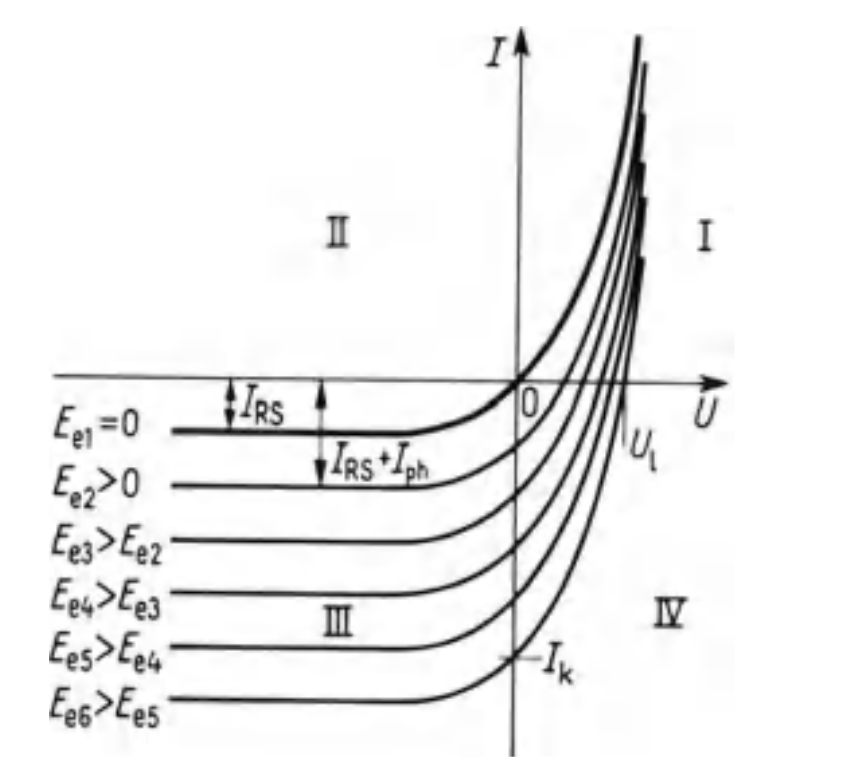
\includegraphics[width=\textwidth]{img/Photodiode-Kennline.png}
    \caption*{Kennlinienfeld $I=f(U)$ der \\Photodiode mit der Bestrah-\\lungsstärke $E_e$ als Parameter\\Kurzschlussstrom $I_k$ bei $U=0$}
    \label{fig:PhotodiodeKennline}
  \end{subfigure}
  %
  \begin{subfigure}[b]{0.6\textwidth}
    \caption{Silizium-Eindringtiefe-Licht}
    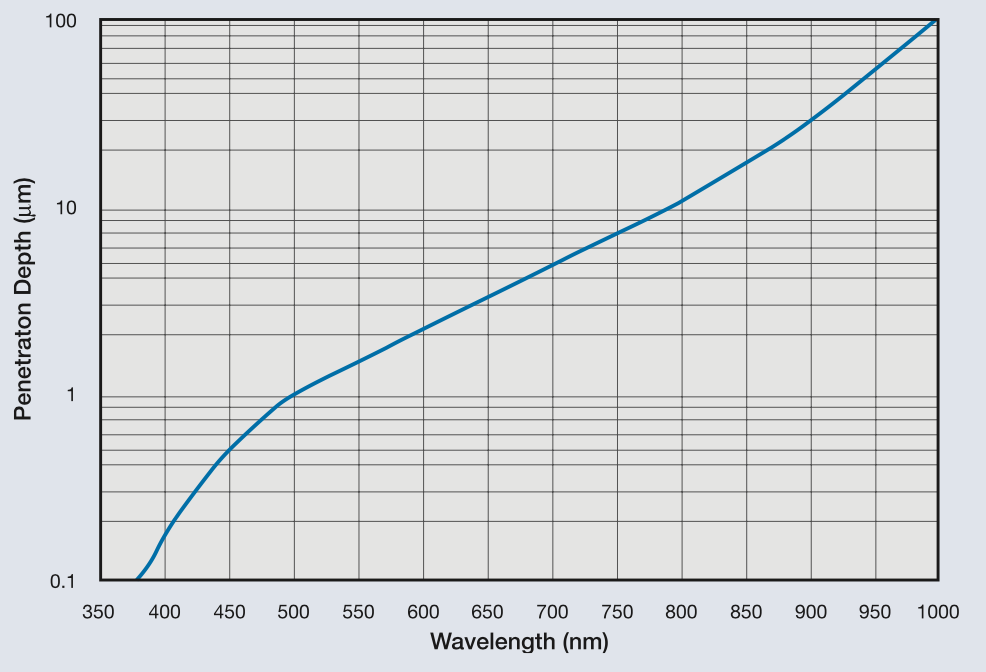
\includegraphics[width=\textwidth]{img/Silizium-Eindringtiefe-Licht.png}
    \caption*{Quelle: osioptoelectronics.com}
  \label{fig:Silizium-eindingtiefe}
  \end{subfigure}
\end{figure}







\noindent Damit Rückschlüsse über den Kurzschlussstrom $I_K$ zur Lichtintensität zulässig sind, muss also die Temperatur konstant oder zumindest bekannt sein.
Außerdem ist es wichtig, bei Tageslichtmessungen, dass einfallende Licht auf eine möglichst begrenzten Wellenlängenbereich zu beschränken, da so ein möglichst akkurater Temperatur und Frequenzabhäniger kompensations faktor gewählt werden kann.
%\subsection{Analog Digital Wanlder}
\subsection{I2C}
I2C ist ein siples und effizentes Busprotokoll.
Es wurde ursprünglich von phillips entwikelt, wird aber seit einigen jahren von NPX weiterentwikelt.
In seiner simpelsten form ermöglicht es einen Master mit bis zu 128 Slave geräten zu verbinden.
Dafür werden nur 2 leitungen benötigt, die die SCL und SDA genannt werden. SCL ist die Taktleitung. Sie wird verwendet, um alle Datenübertragungen über den I2C-Bus zu synchronisieren. SDA ist die Datenleitung.
Außerdem müssen alle Bus teilnehmer mit dem gleichen GND potential verbunden sein um stromfluss über SDA und SCL leitungen zu ermöglichen.


Da SCL und SDA als “open drain” betrieben werden, was bedeutet das die Bus teilnehmer den output low aber nicht high setzen können, muss ein Pull up Wiederstand zur versorgungspannung verwendet werden.

Die Clock leitung SCL wird nur vom Bus Master gesteuert.
Die SDA leitung wird vom Master und Slave genutzt allerdings antworten die Slaves im normalbetrieb nur nachdem sie vom master auf iherer Adresse eine Anfrage erhalten haben. 
Die Spezifikation des Protokolls empfiehlt die SDA und SCL Leitung möglichst weit voneinander zu entfernen um so die Signalqualität zu verbessern.

